\documentclass[
  12pt,
  openright,
  oneside,
  a4paper,
  brazilian
]{abntex2}

\usepackage[T1]{fontenc}
\usepackage[utf8]{inputenc}
\usepackage{newtxtext,newtxmath}
\usepackage{indentfirst}
\usepackage{graphicx}
\usepackage{booktabs}
\usepackage{float}
\usepackage{microtype}
\usepackage{caption}
\usepackage{subcaption}
\usepackage{chngcntr}
\usepackage{setspace}
\usepackage{geometry}
\usepackage{fancyhdr}
\usepackage[alf]{abntex2cite}
\graphicspath{{./figs/}{./sections/figs/}}

\geometry{
  a4paper,
  top=3cm,
  left=3cm,
  bottom=2cm,
  right=2cm
}

\setlength{\parindent}{1.25cm}
\setlength{\parskip}{0pt}
\OnehalfSpacing

\pagestyle{fancy}
\fancyhf{}
\fancyhead[R]{\thepage}
\renewcommand{\headrulewidth}{0pt}

\DeclareCaptionFont{eventten}{\fontsize{10}{12}\selectfont}
\DeclareCaptionLabelFormat{eventhyphen}{#1~#2 -}

\captionsetup{
  justification=centering,
  font=eventten
}

\captionsetup[figure]{
  name=Figura,
  labelformat=eventhyphen,
  labelsep=none,
  labelfont=normalfont,
  textfont=normalfont,
  font=eventten,
  position=above
}

\captionsetup[table]{
  name=Tabela,
  labelformat=eventhyphen,
  labelsep=none,
  labelfont=normalfont,
  textfont=normalfont,
  font=eventten
}

\counterwithout{section}{chapter}
\setcounter{section}{0}
\setcounter{subsection}{0}
\renewcommand{\thesection}{\arabic{section}}
\renewcommand{\thesubsection}{\thesection.\arabic{subsection}}

\newcommand{\eventsection}[1]{%
  \refstepcounter{section}%
  \setcounter{subsection}{0}%
  \par\addvspace{1.2\baselineskip}%
  \noindent\textbf{\thesection.\ \MakeUppercase{#1}}\par
  \nobreak\vspace{0.7\baselineskip}%
}

\newcommand{\eventsubsection}[1]{%
  \refstepcounter{subsection}%
  \par\addvspace{\baselineskip}%
  \noindent\textbf{\thesubsection\ #1}\par
  \nobreak\vspace{0.5\baselineskip}%
}

\newcommand{\artigofonte}[1]{
  \vspace{0.2cm}
  \begin{center}
    \fontsize{10}{12}\selectfont Fonte: #1
  \end{center}
}

\newcommand{\tabelafonte}{\fontsize{10}{12}\selectfont}
\renewcommand{\bibname}{REFER\^ENCIAS}
\renewcommand{\bibsection}{%
  \par\addvspace{1.2\baselineskip}%
  \noindent\textbf{\MakeUppercase{\bibname}}\par
  \nobreak\vspace{0.7\baselineskip}%
}

\titulo{SISTEMA INTELIGENTE EMBARCADO PARA MONITORAMENTO DA QUALIDADE DA \'AGUA EM REGI\~OES REMOTAS DA AMAZ\^ONIA}
\autor{Submiss\~ao sem identifica\c{c}\~ao de autoria}
\data{2026}

\begin{document}

\begin{center}
{\bfseries\MakeUppercase{\thetitle}}
\end{center}

\begin{center}
\textit{Submiss\~ao sem identifica\c{c}\~ao de autoria}
\end{center}

\begin{center}
\textit{Os dados de autoria, institui\c{c}\~ao e e-mail ser\~ao informados ap\'os a avalia\c{c}\~ao.}
\end{center}

\begin{center}
\textbf{Eixo tem\'atico:} Ci\^encias, Tecnologias e Sa\'ude na Amaz\^onia
\end{center}

\noindent\textbf{Resumo}

\vspace{0.3cm}
\noindent
O monitoramento da qualidade da \'agua em regi\~oes remotas da Amaz\^onia ainda enfrenta limita\c{c}\~oes de acesso, conectividade e custo operacional. Nesse contexto, este trabalho apresenta um sistema inteligente embarcado para apoio ao monitoramento offline da qualidade da \'agua no Lago do Serpa, em Itacoatiara, Amazonas. A proposta utiliza medi\c{c}\~oes georreferenciadas de campo e um modelo de intelig\^encia artificial otimizado para execu\c{c}\~ao local, com predi\c{c}\~ao dos par\^ametros pH, oxig\^enio dissolvido e turbidez. O sistema foi validado em diferentes plataformas de borda, incluindo ESP32, Raspberry Pi e dispositivos Android, sem depend\^encia de nuvem. Os resultados indicaram erro absoluto m\'edio de 0,107 para pH, 0,222 para oxig\^enio dissolvido e 0,971 para turbidez no melhor modelo multimodal, al\'em de infer\^encia com baixa lat\^encia em Raspberry Pi e smartphones e opera\c{c}\~ao vi\'avel em microcontrolador. Conclui-se que a solu\c{c}\~ao apresenta potencial para aplica\c{c}\~ao em comunidades ribeirinhas e em a\c{c}\~oes de vigil\^ancia ambiental, contribuindo para a sa\'ude p\'ublica e para a preserva\c{c}\~ao de ecossistemas amaz\^onicos.

\vspace{0.5cm}
\noindent\textbf{Palavras-Chaves:} qualidade da \'agua; Amaz\^onia; intelig\^encia artificial embarcada; monitoramento ambiental; intelig\^encia artificial de borda.

\vspace{0.8cm}

\eventsection{INTRODU\c{C}\~AO}

Na Amaz\^onia, a rela\c{c}\~ao entre popula\c{c}\~oes locais e os ambientes aqu\'aticos \'e imediata. Lagos, rios e igarap\'es sustentam deslocamentos, abastecimento, pesca, atividades produtivas e rotinas comunit\'arias, especialmente em territ\'orios ribeirinhos. Por essa raz\~ao, altera\c{c}\~oes na qualidade da \'agua podem gerar impactos ambientais e sociais relevantes, atingindo tanto o equil\'ibrio ecol\'ogico quanto as condi\c{c}\~oes de vida das comunidades que dependem desses recursos.

Apesar dessa import\^ancia, o acompanhamento sistem\'atico da qualidade da \'agua ainda enfrenta barreiras pr\'aticas. Em muitas \'areas amaz\^onicas, as campanhas de coleta s\~ao espa\c{c}adas, o acesso aos pontos de medi\c{c}\~ao exige deslocamentos longos e a conectividade digital \'e inst\'avel ou inexistente. Nesse cen\'ario, solu\c{c}\~oes apoiadas apenas em transmiss\~ao cont\'inua de dados para servi\c{c}os remotos tendem a apresentar limita\c{c}\~oes operacionais e financeiras. A literatura aponta que sistemas baseados em Internet das Coisas e intelig\^encia artificial podem ampliar a capacidade de monitoramento, mas sua efic\'acia depende de adapta\c{c}\~ao \`as condi\c{c}\~oes reais de rede, log\'istica e uso em campo \cite{zulkifli2022,rahu2023,lowe2022}. Esse contexto favorece abordagens capazes de processar informa\c{c}\~oes no pr\'oprio local de uso. A intelig\^encia artificial de borda surge como alternativa promissora ao permitir infer\^encia local, menor depend\^encia de internet e maior autonomia dos dispositivos, caracter\'isticas valiosas para a realidade amaz\^onica \cite{aral2024}. \'E nesse horizonte que se insere este trabalho, voltado a solu\c{c}\~oes tecnol\'ogicas de baixo custo ajustadas \`a realidade amaz\^onica.

Neste artigo, apresenta-se uma proposta aplicada para o Lago do Serpa, em Itacoatiara, Amazonas, com foco no monitoramento offline de pH, oxig\^enio dissolvido e turbidez. A \^enfase n\~ao recai sobre o detalhamento interno da modelagem, mas sobre a demonstra\c{c}\~ao de uso de um sistema embarcado capaz de operar em plataformas acess\'iveis e em um cen\'ario territorial concreto.

Do ponto de vista do eixo tem\'atico do evento, a relev\^ancia da proposta est\'a em aproximar tecnologia e necessidade social. Em vez de tratar a qualidade da \'agua apenas como um problema de laborat\'orio ou de alto desempenho computacional, o estudo a enquadra como tema de vigil\^ancia ambiental, preven\c{c}\~ao de riscos e apoio \`a tomada de decis\~ao em regi\~oes remotas. Este trabalho deriva de um estudo anterior voltado \`a modelagem e \`a avalia\c{c}\~ao t\'ecnica de intelig\^encia artificial embarcada. Nesta vers\~ao, a prioridade recai sobre a aplica\c{c}\~ao pr\'atica, a leitura territorial dos resultados e o contexto socioambiental amaz\^onico. A principal contribui\c{c}\~ao deste trabalho est\'a na demonstra\c{c}\~ao de um sistema funcional, embarcado e offline, validado em m\'ultiplas plataformas e aplicado a um cen\'ario real da Amaz\^onia. Nesse sentido, a proposta se apresenta como alternativa para monitoramento ambiental de baixo custo, apoio \`a sa\'ude p\'ublica e suporte a comunidades ribeirinhas em regi\~oes remotas.

As principais contribui\c{c}\~oes deste trabalho podem ser sintetizadas em quatro pontos: o desenvolvimento de um sistema embarcado para monitoramento da qualidade da \'agua; a valida\c{c}\~ao da solu\c{c}\~ao em m\'ultiplas plataformas acess\'iveis; a demonstra\c{c}\~ao de aplicabilidade em um cen\'ario real da Amaz\^onia; e a proposi\c{c}\~ao de um uso voltado ao monitoramento ambiental de baixo custo em regi\~oes de baixa conectividade.

\eventsection{FUNDAMENTA\c{C}\~AO TE\'ORICA}

O monitoramento da qualidade da \'agua normalmente considera vari\'aveis como pH, oxig\^enio dissolvido e turbidez, pois esses indicadores ajudam a identificar altera\c{c}\~oes ambientais e condi\c{c}\~oes que podem afetar a vida aqu\'atica e o uso humano da \'agua. No contexto brasileiro, esses par\^ametros tamb\'em s\~ao amplamente empregados como refer\^encia em processos de avalia\c{c}\~ao e gest\~ao de recursos h\'idricos \cite{conama3572005}.

Nos \'ultimos anos, a aplica\c{c}\~ao de intelig\^encia artificial ao monitoramento ambiental cresceu de forma significativa. Estudos t\^em mostrado que modelos computacionais podem auxiliar na predi\c{c}\~ao de vari\'aveis de qualidade da \'agua, especialmente quando h\'a rela\c{c}\~oes n\~ao lineares entre os atributos medidos em campo \cite{ahmed2019,aladhaileh2021,yan2024}. Trabalhos com redes neurais artificiais j\'a haviam demonstrado esse potencial em diferentes cen\'arios \cite{palani2008}, e modelos recorrentes baseados em LSTM refor\c{c}aram a capacidade de capturar padr\~oes mais complexos em s\'eries ambientais \cite{liu2019}. 

Em paralelo, revis\~oes recentes destacam o avan\c{c}o de arquiteturas integradas com sensoriamento, comunica\c{c}\~ao e an\'alise local de dados \cite{zulkifli2022}. Estudos com Internet das Coisas e monitoramento em tempo real mostram ganhos de observa\c{c}\~ao e decis\~ao local, como no caso de sistemas com redes de sensores e apoio de aprendizado de m\'aquina aplicados a rios \cite{rosero2020}. Ainda assim, boa parte dessas solu\c{c}\~oes permanece associada a servidores externos, transmiss\~ao de dados e condi\c{c}\~oes de infraestrutura mais est\'aveis do que as encontradas em regi\~oes remotas. Nesse cen\'ario, a intelig\^encia artificial de borda se destaca por realizar o processamento diretamente no dispositivo, favorecendo aplica\c{c}\~oes em contextos de baixa conectividade \cite{aral2024}.

Outro ponto importante \'e que, em cen\'arios ambientais reais, a utilidade de um sistema n\~ao depende apenas de atingir bom desempenho matem\'atico, mas tamb\'em de conseguir funcionar em condi\c{c}\~oes de uso. Em regi\~oes distantes dos grandes centros, o monitoramento da qualidade da \'agua precisa considerar simplicidade de implanta\c{c}\~ao, manuten\c{c}\~ao reduzida e possibilidade de uso por equipes de campo com restri\c{c}\~oes operacionais. Por isso, uma abordagem embarcada pode ser especialmente adequada quando o objetivo n\~ao \'e apenas produzir previs\~oes, mas apoiar decis\~oes locais. Em vez de depender exclusivamente de conectividade cont\'inua, a solu\c{c}\~ao pode entregar respostas diretamente no dispositivo, tornando o monitoramento mais resiliente e mais compat\'ivel com rotinas de uso em lagos, comunidades ribeirinhas e campanhas ambientais.

No caso espec\'ifico da Amaz\^onia, esse enquadramento \'e decisivo. O Lago do Serpa, por exemplo, insere-se em um contexto territorial no qual a rela\c{c}\~ao entre comunidade, ambiente e uso do espa\c{c}o \'e socialmente relevante \cite{nogueira2022}. O ganho principal de uma solu\c{c}\~ao embarcada, nesse caso, n\~ao est\'a necessariamente em superar todos os modelos tradicionais em desempenho absoluto, mas em conseguir transformar intelig\^encia computacional em uma ferramenta de uso pr\'atico em territ\'orios marcados por grandes dist\^ancias, restri\c{c}\~oes de infraestrutura e alta import\^ancia socioambiental dos corpos h\'idricos.

Assim, a base conceitual deste trabalho articula tr\^es pontos principais: a import\^ancia dos indicadores de qualidade da \'agua, o potencial da intelig\^encia artificial para apoiar diagn\'osticos ambientais e a relev\^ancia de solu\c{c}\~oes embarcadas e offline para regi\~oes remotas. Em vez de competir por maior sofistica\c{c}\~ao algor\'itmica, o estudo prioriza a aplica\c{c}\~ao pr\'atica e a viabilidade de uso em um cen\'ario amaz\^onico real.

\begin{table}[H]
\centering
\footnotesize
\setlength{\tabcolsep}{4pt}
\caption{Lacunas da literatura e posicionamento do presente trabalho.}
\label{tab:gaps_literatura}
\tabelafonte
\begin{tabular}{p{2.8cm}p{4.7cm}p{4.7cm}}
\toprule
Estudo & Foco principal & Lacuna em rela\c{c}\~ao a este trabalho \\
\midrule
Palani et al. \cite{palani2008} & Previs\~ao de vari\'aveis de qualidade da \'agua com ANN em ambiente costeiro & O foco recai sobre modelagem preditiva em ambiente costeiro, sem explorar aplica\c{c}\~ao embarcada em contexto amaz\^onico \\
Liu et al. \cite{liu2019} & Predi\c{c}\~ao de qualidade da \'agua pot\'avel com LSTM em ambiente IoT & O foco est\'a em s\'eries temporais e dados de esta\c{c}\~ao autom\'atica, n\~ao em execu\c{c}\~ao offline em dispositivos acess\'iveis \\
Rosero-Montalvo et al. \cite{rosero2020} & Rede WSN com an\'alise local e apoio de servidor para monitoramento de rio & Aproxima-se do uso em campo, mas em rede dedicada e com apoio externo, diferindo da valida\c{c}\~ao multiplataforma adotada aqui \\
Zulkifli et al. \cite{zulkifli2022} & Revis\~ao sistem\'atica sobre monitoramento h\'idrico baseado em IoT & Identifica desafios e tend\^encias gerais, sem se dedicar a um estudo territorial aplicado na Amaz\^onia \\
Aral \cite{aral2024} & Artigo de posicionamento sobre IA de borda para monitoramento rural & Refor\c{c}a a pertin\^encia conceitual da infer\^encia local, sem apresentar valida\c{c}\~ao experimental aplicada como a desenvolvida neste estudo \\
\bottomrule
\end{tabular}
\artigofonte{elabora\c{c}\~ao pr\'opria com base na literatura utilizada na fundamenta\c{c}\~ao te\'orica.}
\end{table}

\eventsection{METODOLOGIA}

\eventsubsection{\'Area de estudo e dados}

O estudo foi desenvolvido a partir de medi\c{c}\~oes realizadas no Lago do Serpa, localizado em Itacoatiara, no estado do Amazonas. O material utilizado foi organizado a partir de pontos georreferenciados de coleta, reunindo informa\c{c}\~oes f\'isico-qu\'imicas da \'agua e atributos associados ao ambiente amostrado, disponibilizados no conjunto de dados georreferenciado publicado em Mendeley Data \cite{assuncao2026dataset}. Neste artigo, o foco recai sobre tr\^es indicadores de interesse para o acompanhamento ambiental: pH, oxig\^enio dissolvido e turbidez.

\begin{figure}[htbp]
\centering
\caption{Caracteriza\c{c}\~ao visual e territorial da \'area de estudo no Lago do Serpa.}
\label{fig:area_estudo}
\begin{subfigure}[t]{0.46\textwidth}
\centering
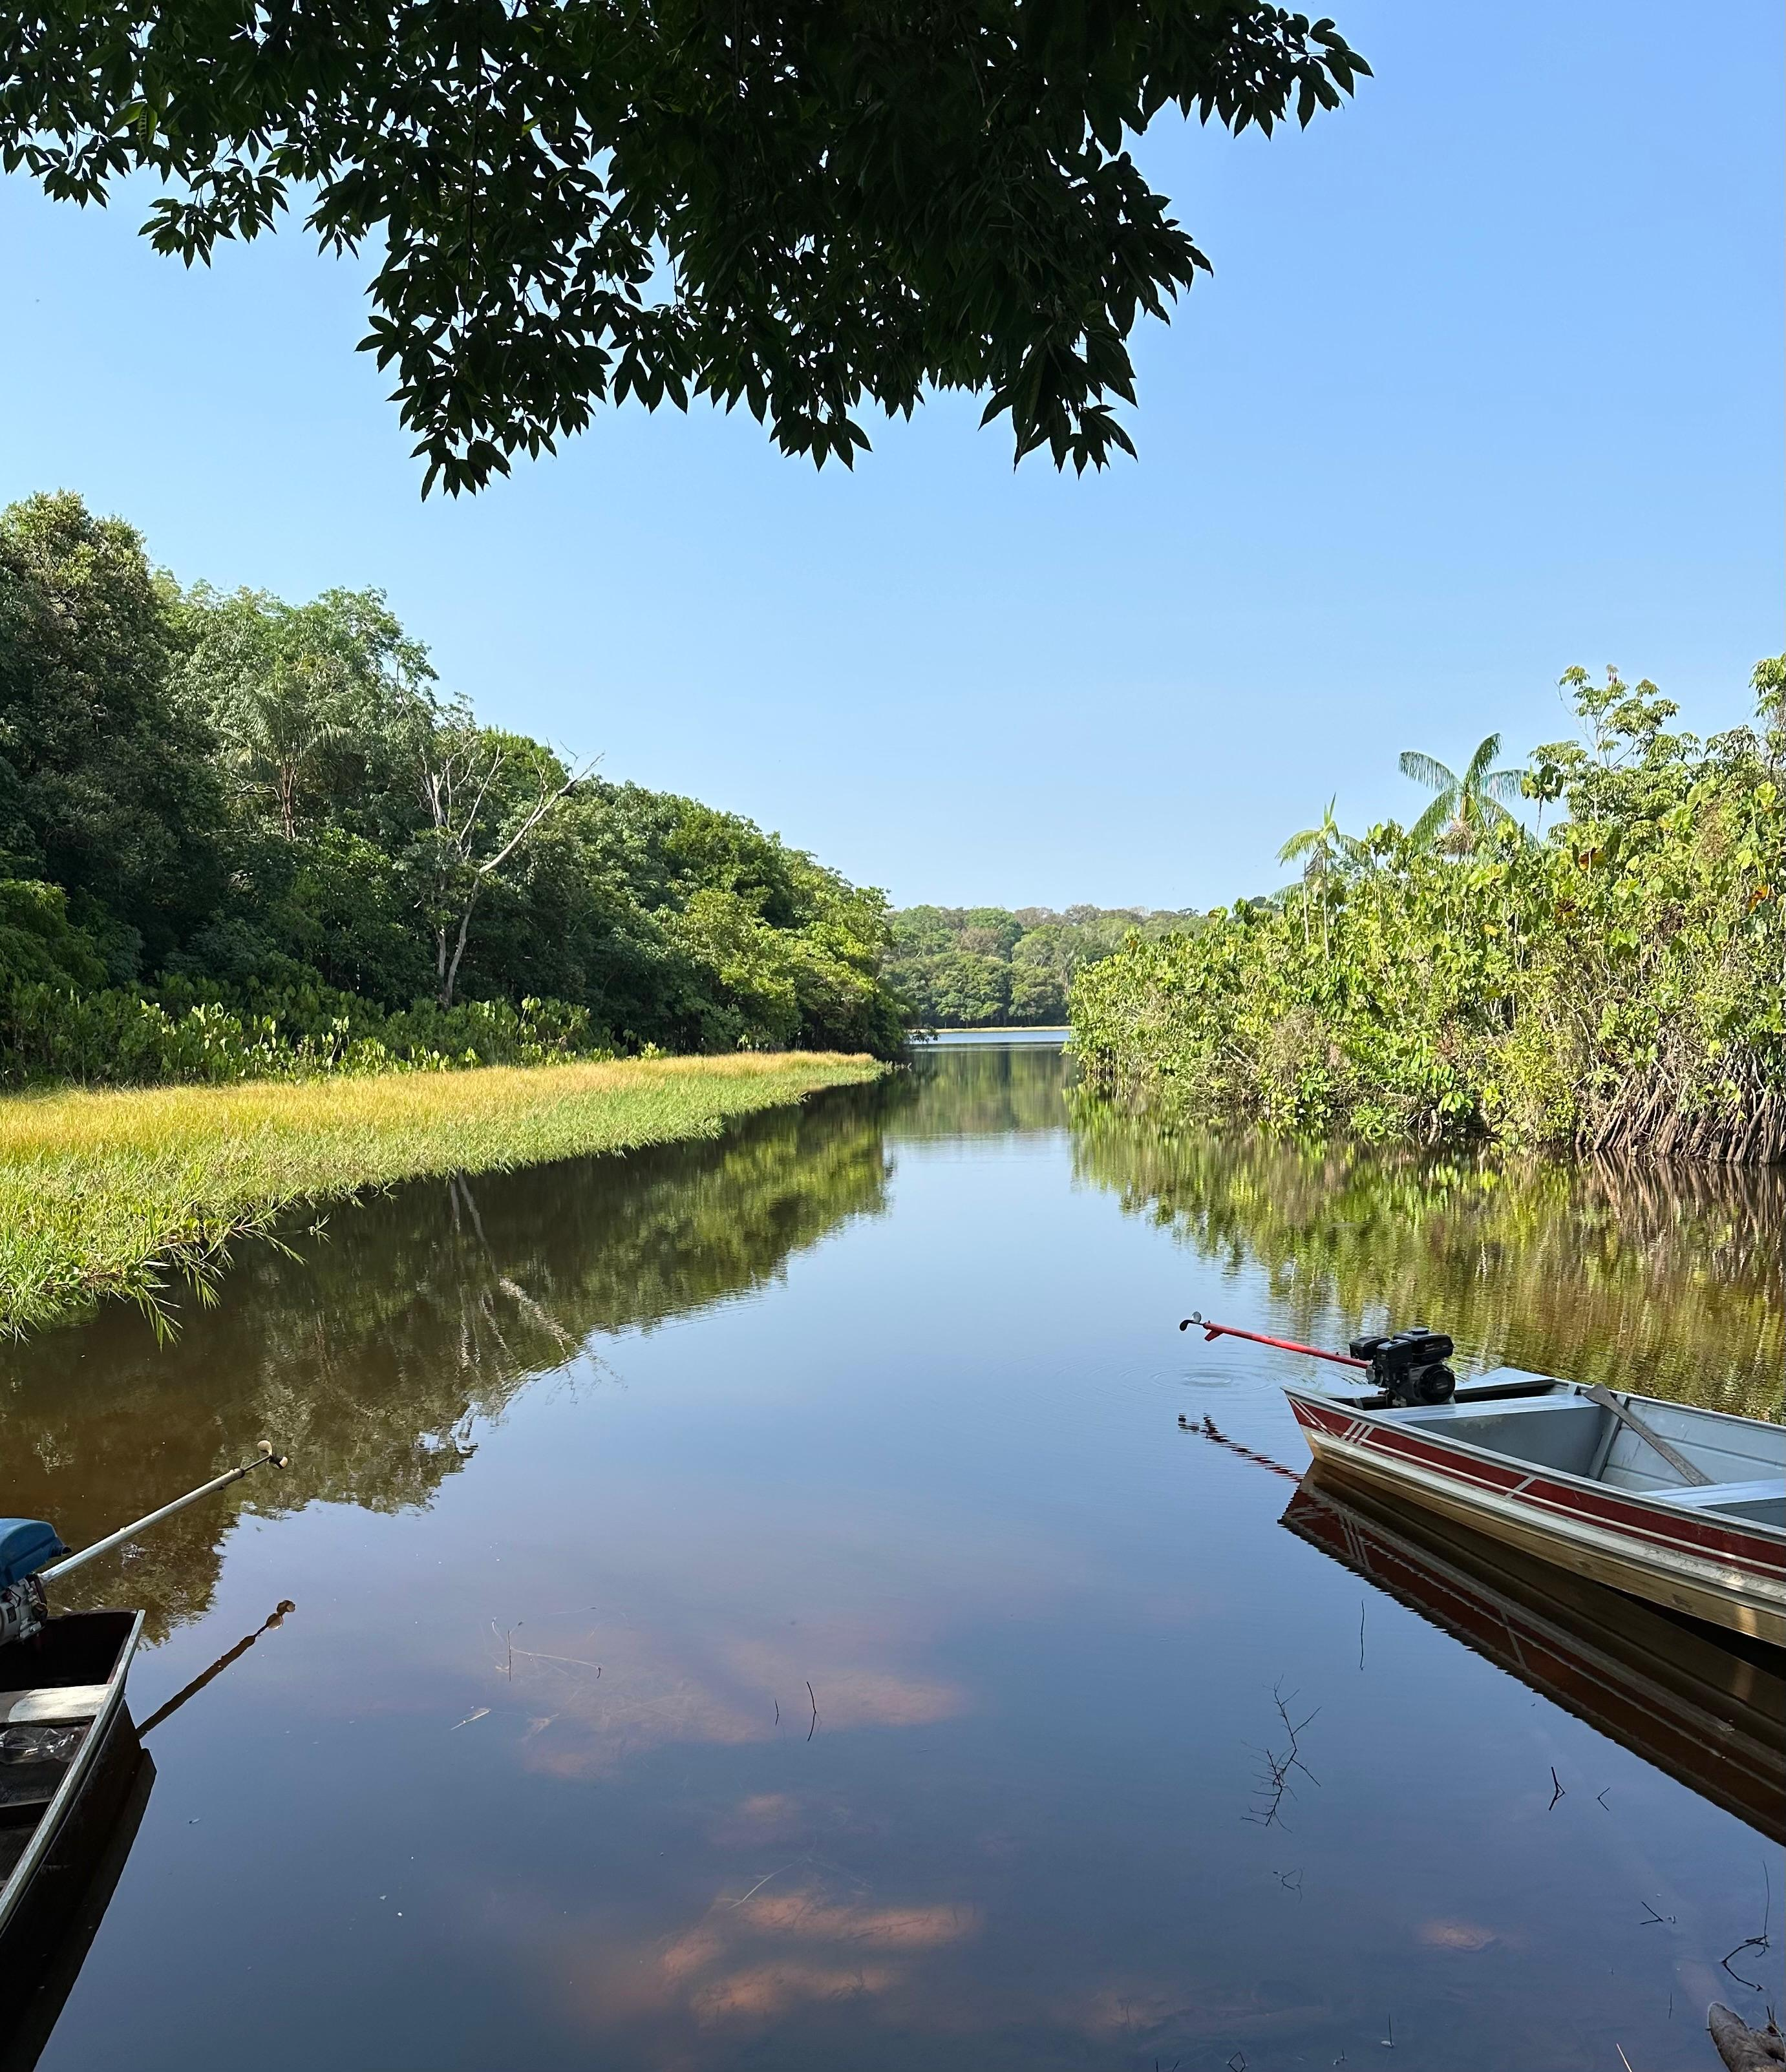
\includegraphics[width=\textwidth]{foto_lago_serpa_clean.jpg}
\caption{Registro visual da \'area estudada}
\end{subfigure}
\hfill
\begin{subfigure}[t]{0.52\textwidth}
\centering
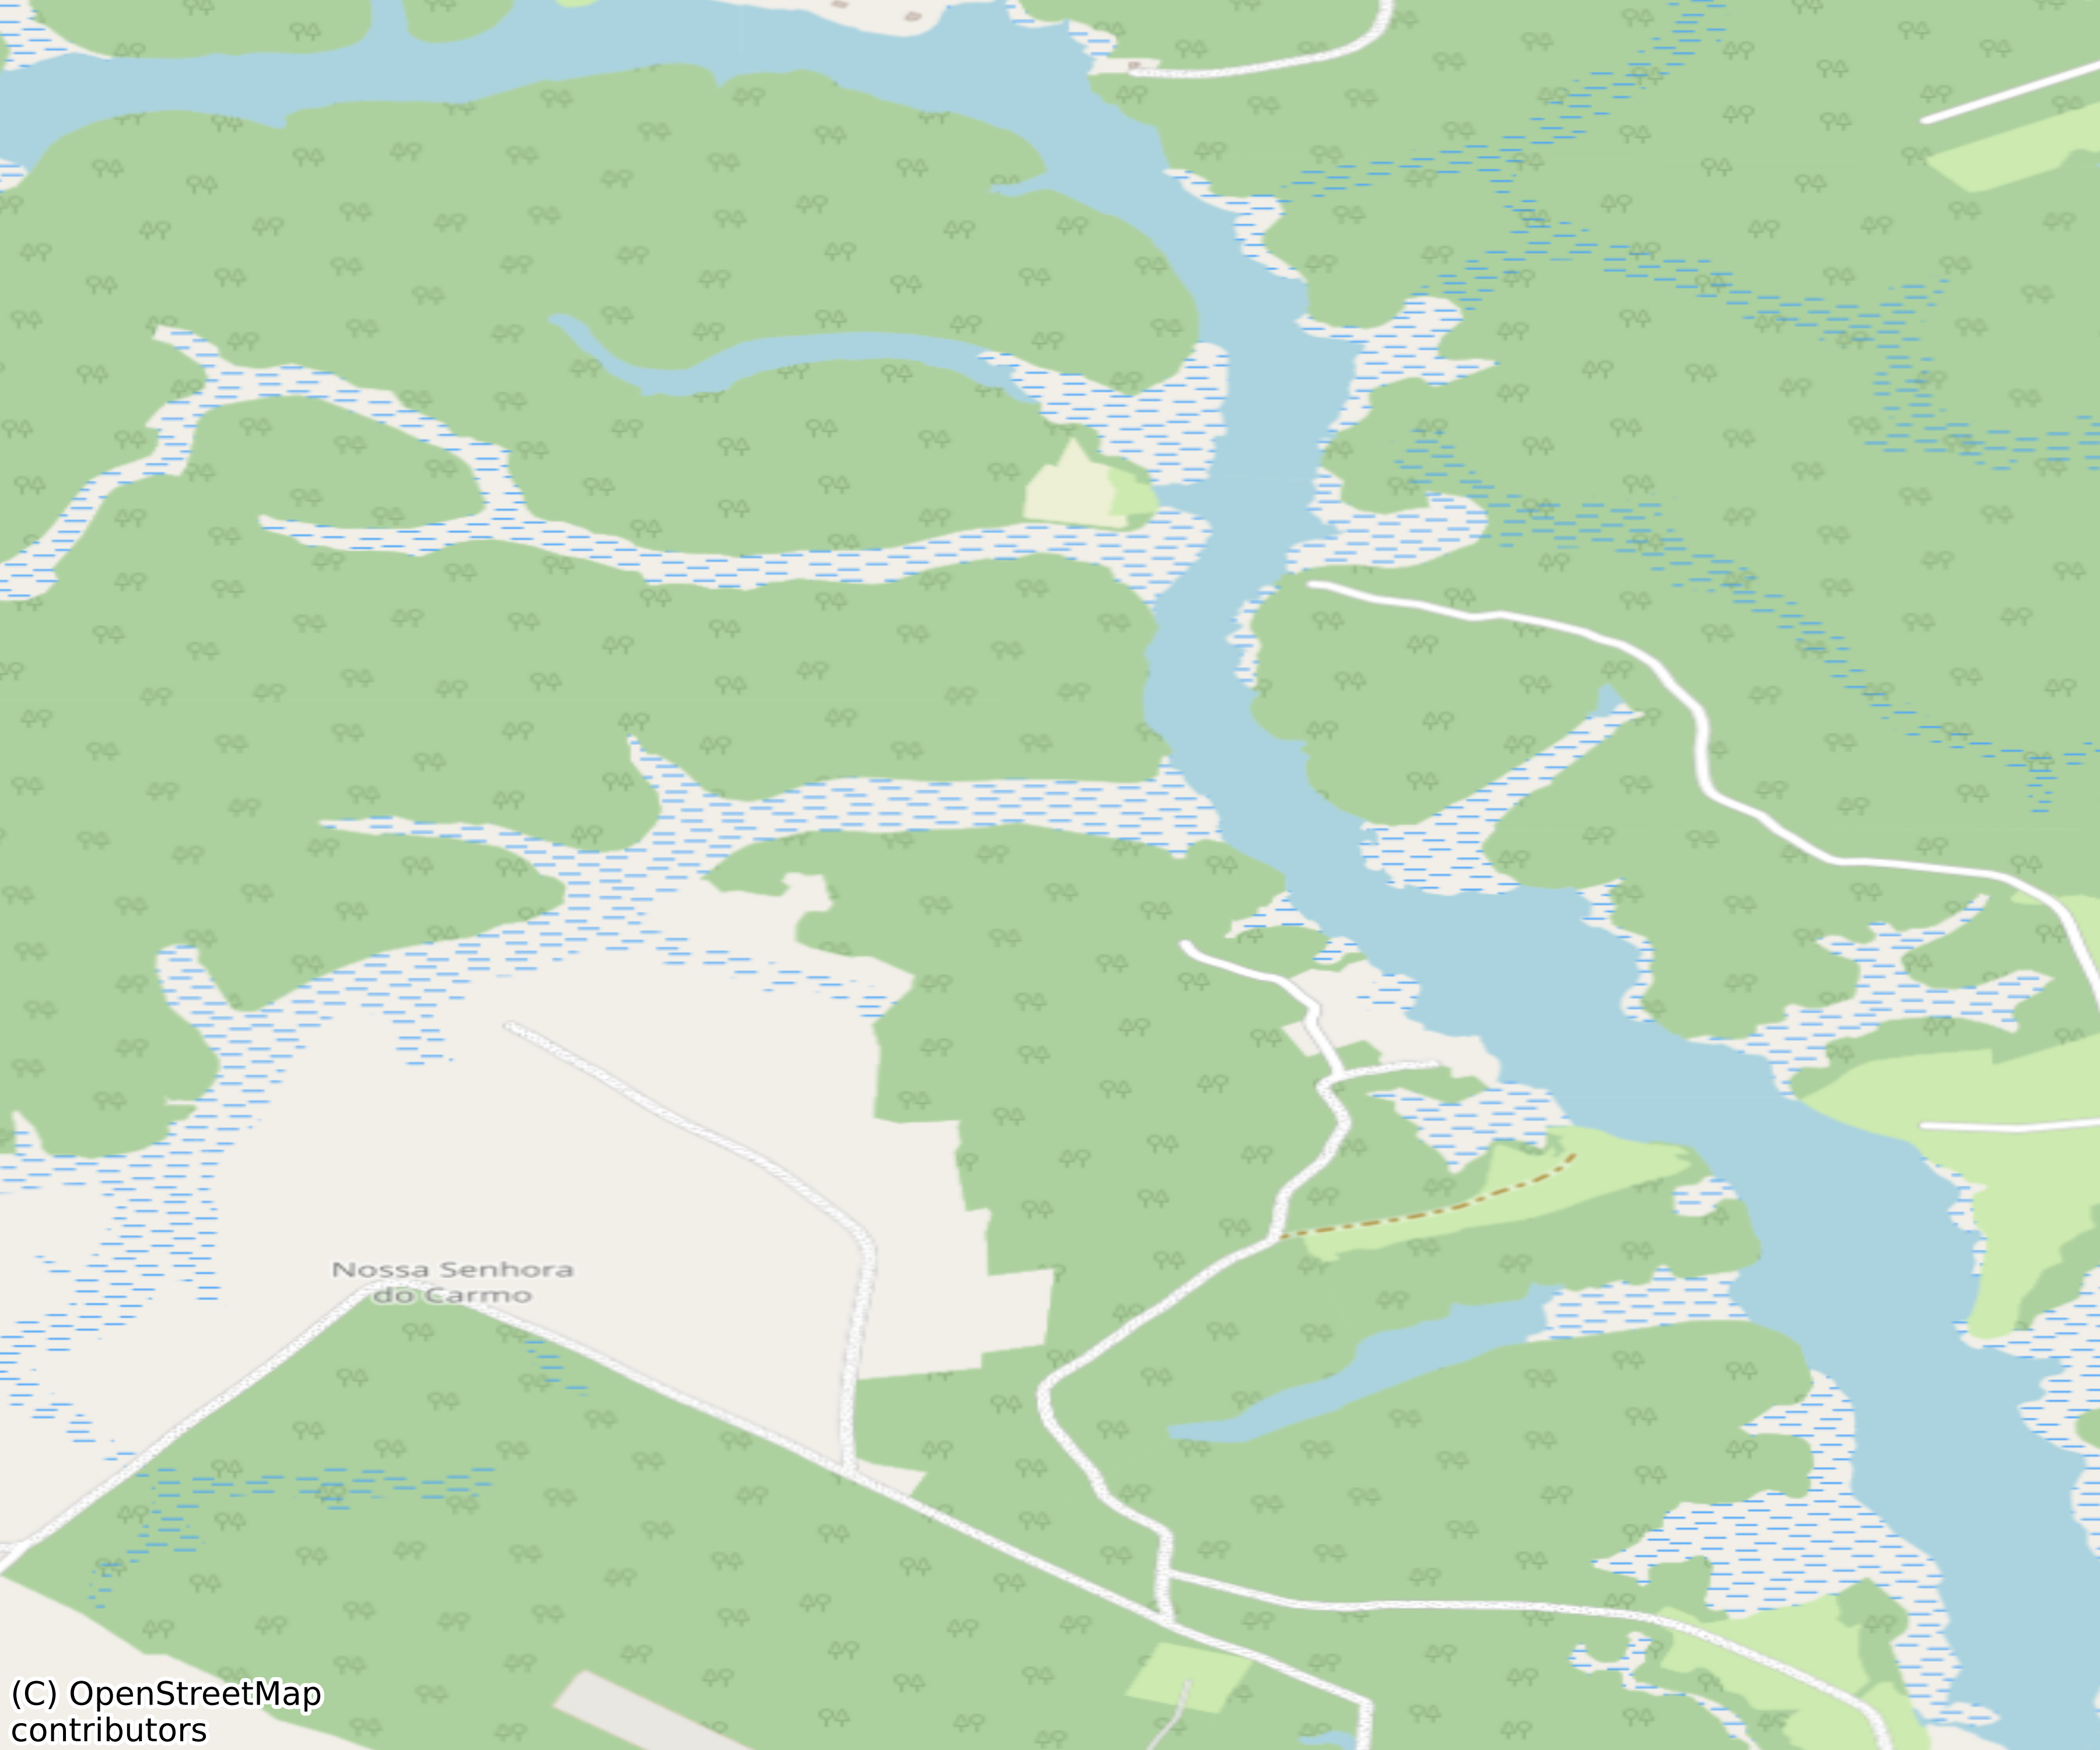
\includegraphics[width=\textwidth]{map_basemap_osm_21S_clean_copy.png}
\caption{Contexto territorial em base cartogr\'afica}
\end{subfigure}
\artigofonte{acervo do estudo de campo e elabora\c{c}\~ao pr\'opria com base em OpenStreetMap.}
\end{figure}

Os dados passaram por etapas de organiza\c{c}\~ao, confer\^encia e padroniza\c{c}\~ao para permitir uso consistente no sistema. Em seguida, o conjunto foi distribu\'ido em etapas de desenvolvimento e verifica\c{c}\~ao da solu\c{c}\~ao, conforme o protocolo adotado no estudo de base. Embora se trate de uma base local, seu valor est\'a no fato de representar um ambiente amaz\^onico real e de permitir a verifica\c{c}\~ao da proposta em condi\c{c}\~oes pr\'oximas do uso em campo.

\eventsubsection{Sistema embarcado proposto}

O sistema proposto foi concebido para funcionar sem depend\^encia de conex\~ao permanente com a internet. Sua l\'ogica de opera\c{c}\~ao pode ser resumida em tr\^es etapas: recebimento dos dados de entrada, processamento local por um modelo de intelig\^encia artificial e apresenta\c{c}\~ao dos resultados ao usu\'ario. Essa organiza\c{c}\~ao permite que o processamento ocorra no pr\'oprio dispositivo, o que \'e especialmente relevante para comunidades ribeirinhas e regi\~oes remotas com baixa conectividade.

Para verificar a viabilidade da proposta, o sistema foi preparado para execu\c{c}\~ao em diferentes plataformas de borda. Foram considerados dispositivos com perfis distintos de uso: smartphones Android, voltados \`a intera\c{c}\~ao em campo; Raspberry Pi, adequada a esta\c{c}\~oes locais de monitoramento; e ESP32, representando um cen\'ario de hardware compacto e de baixo custo.

Essa variedade de plataformas permite observar a solu\c{c}\~ao em condi\c{c}\~oes pr\'aticas distintas. Em um cen\'ario, a prioridade pode ser a visualiza\c{c}\~ao local e a facilidade de uso; em outro, pode ser a implanta\c{c}\~ao em dispositivos pequenos e simples. Assim, a metodologia foi estruturada para avaliar a capacidade de adapta\c{c}\~ao do sistema a diferentes rotinas de monitoramento ambiental, sem concentrar a discuss\~ao em detalhes internos do modelo.

\eventsubsection{Procedimentos de avalia\c{c}\~ao}

A avalia\c{c}\~ao foi conduzida em duas frentes complementares. A primeira considerou a capacidade do sistema de estimar os par\^ametros de interesse a partir dos dados dispon\'iveis. A segunda observou sua execu\c{c}\~ao em plataformas embarcadas, levando em conta medidas de lat\^encia e vaz\~ao de infer\^encia. O objetivo n\~ao foi apenas verificar se o sistema produz bons resultados num\'ericos, mas se esses resultados podem ser efetivamente aproveitados em uma rotina de monitoramento ambiental. Dessa forma, a metodologia privilegia uma leitura aplicada: al\'em de prever vari\'aveis, o sistema precisa ser vi\'avel em dispositivos reais e \'util para apoiar acompanhamento cont\'inuo, triagem ambiental, apoio \`a sa\'ude p\'ublica e identifica\c{c}\~ao de \'areas de maior aten\c{c}\~ao em regi\~oes de dif\'icil acesso.

\eventsection{RESULTADOS E DISCUSS\~AO}

Os resultados obtidos indicam que o sistema \'e capaz de apoiar o monitoramento ambiental do Lago do Serpa com respostas num\'ericas consistentes para os par\^ametros analisados. No melhor arranjo avaliado, os erros absolutos m\'edios foram de 0,107 para pH, 0,222 para oxig\^enio dissolvido e 0,971 para turbidez. Em termos pr\'aticos, esses valores mostram que a solu\c{c}\~ao pode apoiar leituras de campo com boa estabilidade para pH e oxig\^enio dissolvido, enquanto a turbidez exige interpreta\c{c}\~ao mais cautelosa, mas ainda \'e \'util para triagem ambiental e defini\c{c}\~ao de novas coletas.

Essa diferen\c{c}a de comportamento tem implica\c{c}\~ao direta para o uso da ferramenta. Em situa\c{c}\~oes de monitoramento ambiental, resultados mais est\'aveis para pH e oxig\^enio dissolvido oferecem suporte importante para acompanhamento das condi\c{c}\~oes da \'agua e para a comunica\c{c}\~ao com equipes locais. No caso da turbidez, embora a incerteza seja maior, a resposta do sistema permanece \'util como indicador de alerta e como apoio \`a tomada de decis\~ao em regi\~oes remotas.

\begin{table}[H]
\centering
\caption{Indicadores de desempenho do sistema para os par\^ametros monitorados.}
\label{tab:desempenho}
\tabelafonte
\begin{tabular}{lc}
\toprule
Par\^ametro & Erro absoluto m\'edio \\
\midrule
pH & 0,107 \\
Oxig\^enio dissolvido & 0,222 \\
Turbidez & 0,971 \\
\bottomrule
\end{tabular}
\artigofonte{elabora\c{c}\~ao pr\'opria com base nos experimentos do estudo de base.}
\end{table}

Tomado isoladamente, esse resultado pontual n\~ao responde se o erro obtido \'e efetivamente competitivo. Por essa raz\~ao, o estudo de base tamb\'em comparou o modelo proposto com tr\^es baselines consolidados: Random Forest, LSTM e MLP. A Tabela \ref{tab:baselines} mostra que, em erro macro m\'edio, Random Forest e LSTM apresentaram desempenho preditivo superior no mesmo conjunto de dados, enquanto o MLP exibiu pior comportamento e forte instabilidade. Assim, a leitura correta n\~ao \'e a de superioridade universal da rede espiculada, mas a de uma solu\c{c}\~ao que preserva desempenho competitivo ao mesmo tempo em que viabiliza processamento local em hardware restrito.

\begin{table}[H]
\centering
\caption{Comparativo multissemente entre o modelo proposto e baselines cl\'assicos.}
\label{tab:baselines}
\tabelafonte
\begin{tabular}{lccc}
\toprule
Modelo & MAE macro & RMSE macro & $R^2$ macro \\
\midrule
Random Forest & 0,409 $\pm$ 0,062 & 0,557 $\pm$ 0,086 & 0,335 $\pm$ 0,131 \\
LSTM & 0,428 $\pm$ 0,059 & 0,548 $\pm$ 0,073 & 0,313 $\pm$ 0,139 \\
SNN multimodal & 0,447 $\pm$ 0,064 & 0,566 $\pm$ 0,072 & 0,291 $\pm$ 0,146 \\
MLP & 0,781 $\pm$ 0,193 & 0,983 $\pm$ 0,178 & -5,460 $\pm$ 5,220 \\
\bottomrule
\end{tabular}
\artigofonte{elabora\c{c}\~ao pr\'opria com base no benchmark multissemente do estudo de base.}
\end{table}

Essa compara\c{c}\~ao \'e decisiva para interpretar a escolha do modelo. Do ponto de vista estritamente preditivo, a arquitetura espiculada n\~ao superou os melhores baselines nesta base local. Sua justificativa t\'ecnica est\'a na combina\c{c}\~ao entre erro aceit\'avel, infer\^encia offline, compatibilidade com exporta\c{c}\~ao para TFLite e potencial de execu\c{c}\~ao em dispositivos de borda como Android, Raspberry Pi e ESP32. Em cen\'arios remotos, esse compromisso entre desempenho e implantabilidade pode ser mais relevante do que a melhor m\'etrica isolada.

Outro aspecto que merece destaque \'e a robustez. O benchmark com dez sementes independentes mostrou que o SNN apresentou MAE macro de 0,447 $\pm$ 0,064, RMSE macro de 0,566 $\pm$ 0,072 e $R^2$ macro de 0,291 $\pm$ 0,146. Esses desvios-padr\~ao n\~ao eliminam a variabilidade esperada de uma base pequena, mas mostram que o comportamento do modelo n\~ao depende de uma \'unica divis\~ao fortuita dos dados. Em contraste, o MLP apresentou dispers\~ao muito maior, o que refor\c{c}a a import\^ancia de discutir estabilidade experimental e n\~ao apenas o melhor MAE encontrado.

Do ponto de vista estat\'istico, tamb\'em cabe cautela. No teste de sinal pareado entre SNN e Random Forest, n\~ao houve evid\^encia de superioridade global do SNN nas m\'etricas macro ao n\'ivel de 5\% de signific\^ancia. Esse resultado refor\c{c}a que a proposta deve ser defendida principalmente por sua viabilidade operacional e territorial, e n\~ao por uma suposta lideran\c{c}a absoluta em acur\'acia dentro desta base.

A interpreta\c{c}\~ao pr\'atica dos resultados se torna mais clara quando as estimativas s\~ao observadas espacialmente. Em vez de focar apenas na compara\c{c}\~ao entre valores previstos e observados, esta vers\~ao do artigo enfatiza a leitura territorial das condi\c{c}\~oes do lago. Isso torna a discuss\~ao mais compat\'ivel com aplica\c{c}\~oes de monitoramento ambiental.

\begin{figure}[H]
\centering
\caption{Painel espacial reconfigurado dos par\^ametros monitorados no Lago do Serpa. Nos mapas, $x$ representa a coordenada leste e $y$ a coordenada norte no sistema UTM 21S, em metros.}
\label{fig:idw_individual}
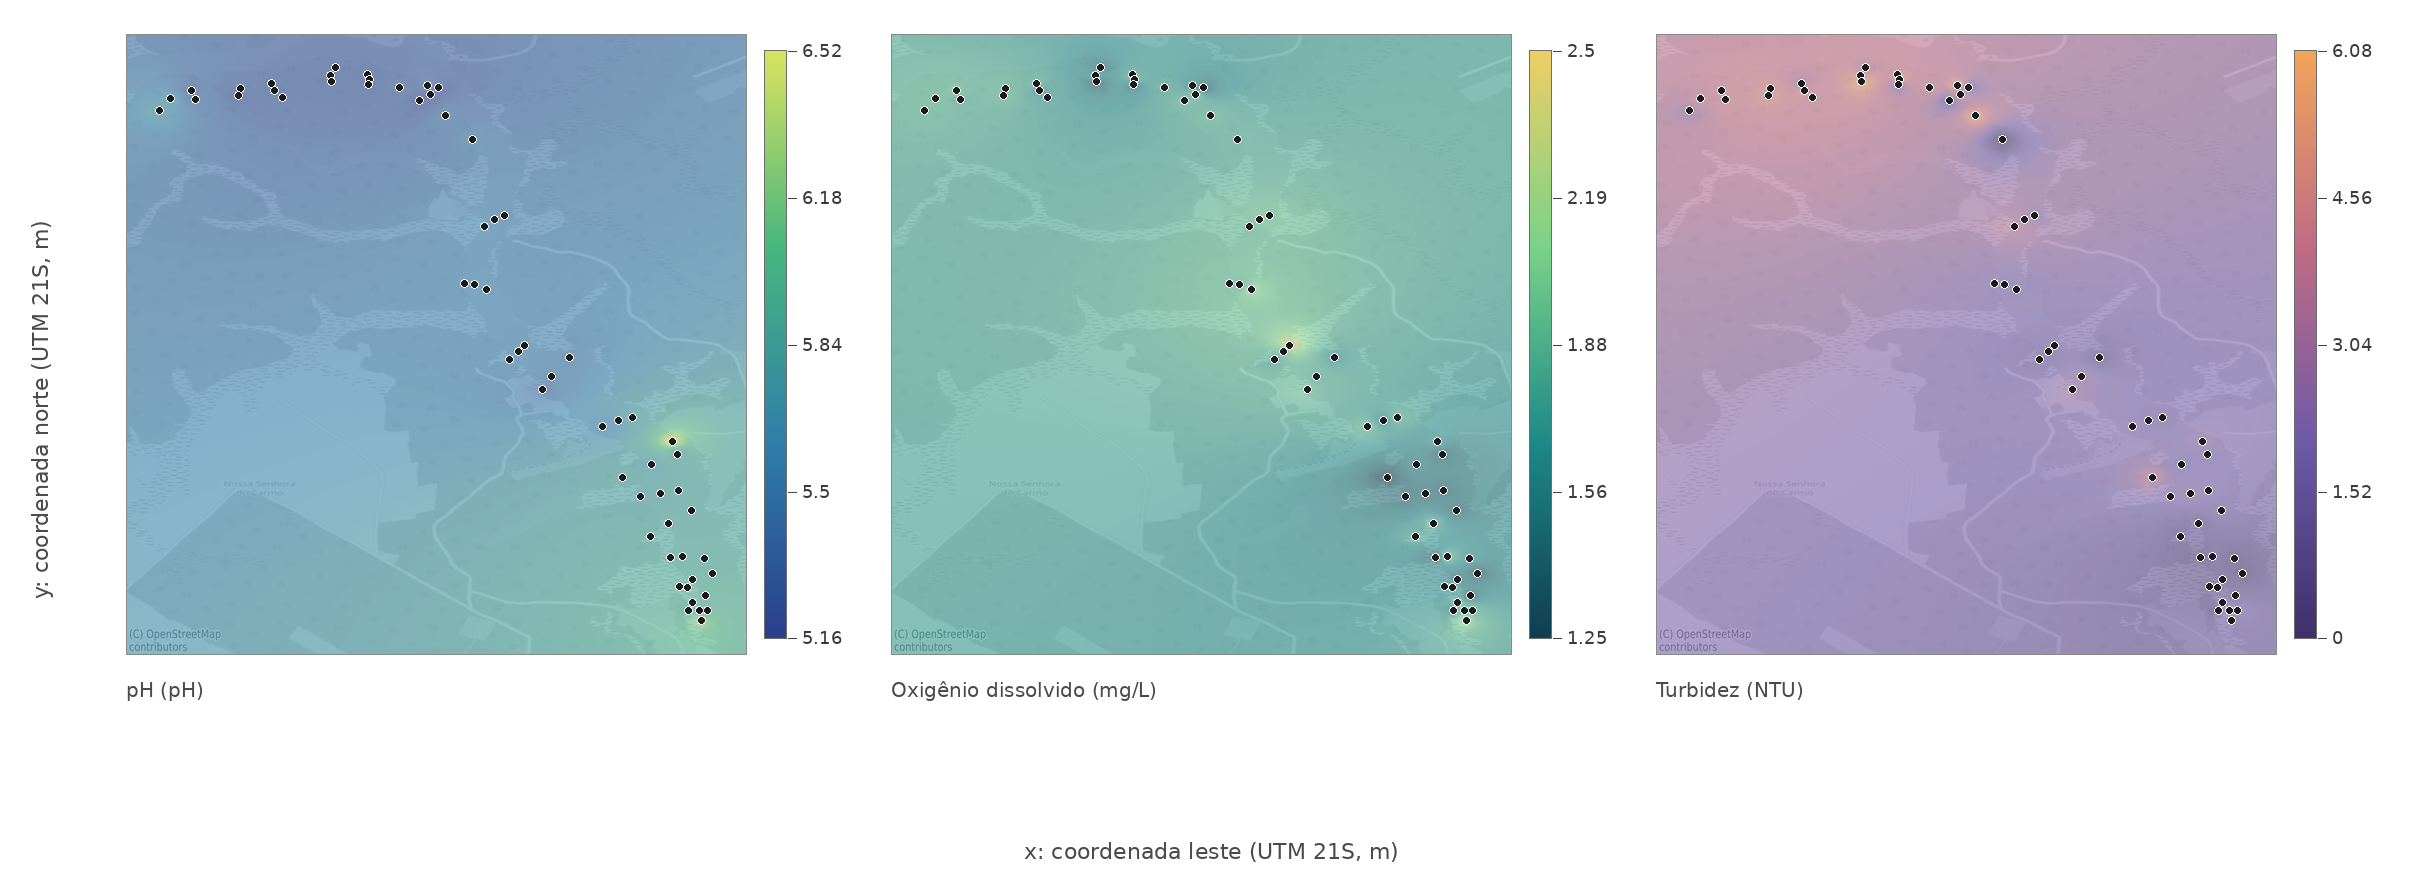
\includegraphics[width=0.98\textwidth]{idw_triptych_redesigned.png}
\artigofonte{elabora\c{c}\~ao pr\'opria com base nas superf\'icies interpoladas do estudo.}
\end{figure}

A Figura \ref{fig:idw_individual} evidencia que a proposta n\~ao se resume \`a gera\c{c}\~ao de valores num\'ericos. Ao produzir uma leitura espacialmente organizada, o sistema contribui para o planejamento de novas coletas, para a comunica\c{c}\~ao dos resultados e para a prioriza\c{c}\~ao de trechos com maior interesse ambiental. Esse tipo de leitura pode ser particularmente relevante para comunidades ribeirinhas e equipes de campo com acesso limitado a laborat\'orios e internet. No que se refere \`a implanta\c{c}\~ao em hardware, a proposta tamb\'em se mostrou vi\'avel. Na Raspberry Pi 4B, a lat\^encia m\'edia foi de 0,214 ms por amostra, com vaz\~ao de 4670,50 amostras por segundo. Em dispositivos Android, os valores foram mais elevados, com destaque para o Device B, que alcan\c{c}ou 30905,08 amostras por segundo. No ESP32, a taxa de 5,0 amostras por segundo indica uma opera\c{c}\~ao mais simples, mas ainda compat\'ivel com monitoramento peri\'odico e aut\^onomo em cen\'arios de baixa conectividade.

\begin{table}[H]
\centering
\caption{Viabilidade operacional do sistema em diferentes plataformas de borda.}
\label{tab:plataformas}
\tabelafonte
\begin{tabular}{lc}
\toprule
Plataforma & Vaz\~ao (amostras/s) \\
\midrule
ESP32 & 5,0 \\
Raspberry Pi 4B & 4670,50 \\
Android A & 12337,40 \\
Android B & 30905,08 \\
Android C & 16121,71 \\
\bottomrule
\end{tabular}
\artigofonte{elabora\c{c}\~ao pr\'opria a partir dos ensaios de execu\c{c}\~ao do sistema.}
\end{table}

Os resultados de execu\c{c}\~ao ajudam, portanto, a distinguir cen\'arios de uso. O ESP32 pode atender a rotinas mais simples e esparsas de monitoramento, o que favorece aplica\c{c}\~oes peri\'odicas e aut\^onomas. J\'a Android e Raspberry Pi oferecem condi\c{c}\~oes mais favor\'aveis quando h\'a necessidade de maior frequ\^encia de processamento, visualiza\c{c}\~ao local, intera\c{c}\~ao com usu\'arios e apoio mais imediato \`a tomada de decis\~ao.

Sob a perspectiva de utilidade social, a leitura espacial dos par\^ametros j\'a oferece valor concreto. Em vez de limitar a interpreta\c{c}\~ao a tabelas t\'ecnicas, o sistema permite uma vis\~ao mais imediata de onde a aten\c{c}\~ao deve ser concentrada. Com isso, o di\'alogo com gestores, equipes de campo, servi\c{c}os de vigil\^ancia ambiental e comunidades locais tende a se tornar mais direto, ampliando o potencial de uso da proposta para al\'em do ambiente estritamente acad\^emico. Outro aspecto relevante \'e a possibilidade de uso progressivo da solu\c{c}\~ao. Em um primeiro momento, o sistema pode funcionar como instrumento complementar de triagem, auxiliando equipes em coletas explorat\'orias e em campanhas pontuais. Em uma etapa posterior, com amplia\c{c}\~ao do conjunto de dados e adapta\c{c}\~ao a outros ambientes aqu\'aticos, a mesma estrutura pode apoiar rotinas mais frequentes de monitoramento territorial.

Esse potencial de expans\~ao \'e importante porque mostra que a proposta n\~ao est\'a restrita a um experimento isolado. Ao contr\'ario, trata-se de uma base tecnol\'ogica que pode ser incrementada em novas campanhas, integrada a outras vari\'aveis ambientais e ajustada a diferentes realidades amaz\^onicas. Mesmo mantendo car\'ater aplicado e de baixo custo, o sistema apresenta perspectiva de continuidade e replicabilidade. Do ponto de vista aplicado, os achados mostram que o sistema pode ser inserido em rotinas de monitoramento em regi\~oes remotas, nas quais a continuidade do acompanhamento depende de solu\c{c}\~oes aut\^onomas, simples e de menor custo. O funcionamento offline amplia o potencial de uso em comunidades ribeirinhas, campanhas de vigil\^ancia ambiental e a\c{c}\~oes de apoio \`a sa\'ude p\'ublica. Ao mesmo tempo, essa interpreta\c{c}\~ao ainda n\~ao equivale a valida\c{c}\~ao externa: como toda a an\'alise foi conduzida com dados do Lago do Serpa, permanece em aberto o desempenho da solu\c{c}\~ao em outros lagos ou contextos amaz\^onicos.

Al\'em disso, o estudo refor\c{c}a um ponto central: o diferencial do artigo n\~ao est\'a em disputar originalidade apenas pelo desenho t\'ecnico do modelo, mas em demonstrar uma aplica\c{c}\~ao concreta e territorialmente situada. Em contextos marcados por baixa conectividade, longas dist\^ancias e forte depend\^encia dos recursos h\'idricos, uma solu\c{c}\~ao embarcada e funcional pode gerar impacto pr\'atico superior ao de abordagens voltadas exclusivamente \`a compara\c{c}\~ao t\'ecnica.

Em s\'intese, os resultados sustentam uma interpreta\c{c}\~ao em duas frentes complementares. A primeira \'e ambiental, ao mostrar que o sistema consegue estimar vari\'aveis relevantes da qualidade da \'agua. A segunda \'e operacional, ao indicar que essa capacidade pode ser levada para dispositivos de campo e convertida em apoio concreto ao monitoramento ambiental, \`a sa\'ude p\'ublica e \`a tomada de decis\~ao na Amaz\^onia.

\eventsubsection{Implica\c{c}\~oes para uso em campo}

Quando se considera o uso do sistema fora do ambiente acad\^emico, alguns pontos ganham destaque. O primeiro deles \'e a possibilidade de reduzir a depend\^encia de processamento remoto em cen\'arios onde a internet \'e limitada. Em muitos territ\'orios amaz\^onicos, a dificuldade n\~ao est\'a apenas em coletar a informa\c{c}\~ao, mas em conseguir transform\'a-la rapidamente em uma leitura \'util para a equipe que est\'a no local. Ao operar no pr\'oprio dispositivo, a solu\c{c}\~ao encurta esse caminho. O segundo ponto est\'a relacionado ao car\'ater progressivo do monitoramento. Em vez de substituir procedimentos tradicionais, o sistema pode atuar como ferramenta complementar, ajudando a indicar onde novas coletas devem ser priorizadas e quais trechos do lago merecem aten\c{c}\~ao mais imediata. Esse tipo de apoio \'e especialmente relevante quando os recursos humanos e log\'isticos s\~ao limitados.

Tamb\'em \'e importante observar que a aplica\c{c}\~ao em campo envolve diferentes perfis de usu\'ario. Pesquisadores, gestores locais, t\'ecnicos ambientais e equipes de apoio podem se beneficiar de uma sa\'ida mais objetiva, baseada em mapas, indicadores e previs\~oes acess\'iveis. Isso amplia a utilidade da proposta, pois a transforma em um recurso de comunica\c{c}\~ao e triagem, n\~ao se tratando, portanto, apenas de uma experi\^encia computacional. Por fim, a experi\^encia com o Lago do Serpa sugere que abordagens desse tipo podem fortalecer estrat\'egias de monitoramento territorial na Amaz\^onia. Mesmo com limita\c{c}\~oes de base de dados, a solu\c{c}\~ao demonstrou que \'e poss\'ivel integrar medi\c{c}\~oes locais, processamento embarcado e leitura espacial em uma estrutura tecnol\'ogica coerente com as condi\c{c}\~oes de regi\~oes remotas, embora a generaliza\c{c}\~ao para outros corpos h\'idricos ainda dependa de valida\c{c}\~ao adicional.

\eventsection{CONSIDERA\c{C}\~OES FINAIS}

Este trabalho apresentou um sistema inteligente embarcado para monitoramento da qualidade da \'agua no contexto amaz\^onico, com aplica\c{c}\~ao no Lago do Serpa, em Itacoatiara, Amazonas. A proposta mostrou ser capaz de operar de forma offline, prever pH, oxig\^enio dissolvido e turbidez e executar processamento em diferentes plataformas de borda, incluindo ESP32, Raspberry Pi e smartphones Android. Os resultados permitem concluir que a solu\c{c}\~ao \'e operacionalmente vi\'avel e socialmente relevante para regi\~oes com baixa infraestrutura de comunica\c{c}\~ao. Seu uso potencial em comunidades ribeirinhas e em a\c{c}\~oes de acompanhamento ambiental pode contribuir para monitoramento cont\'inuo, apoio \`a tomada de decis\~ao e fortalecimento de estrat\'egias de preserva\c{c}\~ao e sa\'ude p\'ublica.

Tamb\'em se destaca que a proposta valoriza um caminho de inova\c{c}\~ao adequado \`a realidade regional. Em vez de depender de estruturas complexas e de alto custo, o sistema busca entregar intelig\^encia computacional em um formato compat\'ivel com o trabalho de campo. Essa escolha torna a solu\c{c}\~ao mais pr\'oxima de cen\'arios reais de uso e mais alinhada com demandas de territ\'orios remotos da Amaz\^onia e de regi\~oes marcadas por baixa conectividade.

A contribui\c{c}\~ao principal deste artigo est\'a justamente nesse deslocamento de foco: do detalhamento da modelagem para a demonstra\c{c}\~ao de aplicabilidade. Ao enfatizar o uso pr\'atico, a opera\c{c}\~ao offline e a relev\^ancia territorial da proposta, o trabalho se apresenta como uma contribui\c{c}\~ao voltada \`a ado\c{c}\~ao de tecnologia de baixo custo em monitoramento ambiental amaz\^onico. Os resultados comparativos tamb\'em mostram que a defesa da arquitetura espiculada deve ser feita com precis\~ao: ela n\~ao foi a melhor baseline em erro m\'edio nesta base, mas se mostrou competitiva e, ao mesmo tempo, compat\'ivel com execu\c{c}\~ao local em diferentes plataformas de borda. Como limita\c{c}\~ao, o estudo ainda depende de uma base de dados local e relativamente reduzida, o que indica a necessidade de ampliar campanhas de coleta em diferentes per\'iodos e ambientes. Como continuidade, recomenda-se expandir a valida\c{c}\~ao em outros corpos h\'idricos amaz\^onicos, incorporar novas vari\'aveis ambientais e aprofundar o uso da solu\c{c}\~ao em cen\'arios reais de monitoramento territorial.

Por fim, entende-se que o principal valor do trabalho est\'a em demonstrar uma ponte entre pesquisa aplicada, tecnologia embarcada e relev\^ancia socioambiental. Ao mostrar que o monitoramento da qualidade da \'agua pode ser realizado de forma offline, local e com potencial de uso em regi\~oes isoladas, o estudo oferece uma contribui\c{c}\~ao concreta para a discuss\~ao sobre tecnologias sustent\'aveis voltadas \`a Amaz\^onia.


\postextual
\bibliography{referencias}

\end{document}
